% to choose your degree
% please un-comment just one of the following
\documentclass[bsc,twoside,singlespacing,parskip,logo,notimes,normalheadings]{infthesis}
% for BSc, BEng etc.

\usepackage[super]{natbib}
\setcitestyle{square}

\usepackage[toc]{appendix}

\usepackage[acronym,section,numberedsection=autolabel]{glossaries}

\makeglossaries

%% Basics
\newglossaryentry{controlflowgraph}
{
        name=control-flow graph,
        description={A graph representing the possible execution paths
        in a program. Nodes represent instructions, edges represent
        possible jumps between said instructions}
}

\newglossaryentry{dataflowanalysis}
{
        name=data-flow analysis,
        description={A technique for gathering information at various
          points in a \gls{controlflowgraph}}
}
 
\newglossaryentry{dataflow}
{
        name=data-flow,
        description={A system of equations and conditions which
          constitute a data-flow problem, that is, a problem which may
          be solved through data-flow analysis}
}

\newglossaryentry{direction}
{
        name=direction,
        description={The direction in which data flows in a
          \gls{dataflow} problem. Either forward (from the entry point
          of the \gls{cfg} to the exit point) or backward (the opposite)}
}

\newglossaryentry{dataflowequations}
{
        name=data-flow equations,
        description={A system of equations which determine how data
          flows through a \gls{cfg}}
}

\newglossaryentry{transfer}
{
        name=transfer,
        description={An equation (or set of equations) which
          determines how data flows {\em through} a node in a \gls{cfg}}
}

\newglossaryentry{meet}
{
        name=meet,
        description={An equation (or set of equations) which
          determines how data flows {\em between} nodes in a \gls{cfg}}
}

%%Graph Theory

\newglossaryentry{region}
{
        name=region,
        description={A set of nodes in a graph which includes a {\em header} node which \gls{dominate}s all other nodes in the region\cite[p. 669]{dragonbook}}
}

\newglossaryentry{dominate}
{
        name=dominate,
        description={In a \gls{cfg} a node $n_i$ is said to dominate a node $n_j$ if every path from $n_0$ (the entry node) to $n_j$ must go through $n_i$\cite[p. 478]{eac}}
}

%%Generic Frameworks 
\newglossaryentry{hassediagram}
{
        name=Hasse diagram,
        description={A diagram used to represent partially ordered
          sets. Nodes represent elements of the sets, edges represent
          an ordering between a pair of elements}
}

\newglossaryentry{meetsemilattice}
{
        name=meet semi-lattice,
        description={A partially ordered set in which there exists a
          greatest lower bound (or meet) for any non-empty, finite subset}
}

\newglossaryentry{meetoperator}
{
        name=meet operator,
        description={An operator which defines how the meet of two
          sets is obtained, such as $\cup$, $\cap$ or another operator
        entirely}
}

\newglossaryentry{domain}
{
        name=domain,
        description={The domain of values considered in a
          \gls{dataflow} problem, e.g. definitions or expressions}
}

\newglossaryentry{boundary}
{
        name=boundary,
        description={The initial value at the starting point of an
          analysis, i.e. $\text{In}(ENTRY)$ or $\text{Out}(EXIT)$}
}

\newglossaryentry{fixedpoint}
{
        name=fixed-point,
        description={A computation in which the required process is
          repeated until the state stops changing}
}



%% Types of Analysis
\newglossaryentry{reachingdefinition}
{
        name=reaching definition,
        description={A definition of a variable {\em reaches} a block if there exists at least one path from its definition to the block along which it is not overwritten}
}

\newglossaryentry{livenessanalysis}
{
        name=liveness analysis,
        description={A variable is {\em live} if its current value will be used later in the program's execution}
}

\newglossaryentry{availableexpression}
{
        name=available expression,
        description={An expression is {\em available} if it has been computed along all paths leading to the current node}
}

%% Evaluation
 
\newglossaryentry{likertscale}
{
        name=Likert scale,
        description={A method of gauging opinion on a topic,
consisting of a collection of Likert items. Each Likert item contains
a statement followed by an odd number of responses, containing an
equal number of positive and negative responses balanced such that the
difference between responses is uniform. An example Likert item is the
oft-used Strongly Agree / Strongly Disagree scale, which may be
weighted from from 1-5. The Likert scale is the sum of weights of
responses to Likert items}
}


%% Acronyms
\newacronym{cfg}{CFG}{control-flow graph}
\newacronym{ast}{AST}{abstract syntax tree}
\newacronym{api}{API}{application programming interface}
\glsunset{api}
\newacronym{es6}{ES6}{ECMAScript 6}
\newacronym{copt}{COPT}{Compiler Optimisations}

%% Text
\usepackage{color}
\usepackage[hyphens]{url}
\renewcommand{\labelitemii}{$\circ$}

%% Math
\usepackage{amsmath}

%% Figures
\usepackage{caption}
\captionsetup{%
  figurename=fig.,
  tablename=tab.
}
\usepackage{capt-of}
\usepackage{wrapfig}
\usepackage[bottom]{footmisc}
\usepackage[absolute,overlay]{textpos}
  \setlength{\TPHorizModule}{1mm}
  \setlength{\TPVertModule}{1mm}

\usepackage{listings}

%% Algorithm listings
\newcounter{nalg}[chapter] % defines algorithm counter for chapter-level
\renewcommand{\thenalg}{\thechapter .\arabic{nalg}} %defines appearance of the algorithm counter
\DeclareCaptionLabelFormat{algocaption}{Algorithm \thenalg} % defines a new caption label as Algorithm x.y

\lstnewenvironment{algorithm}[1][] %defines the algorithm listing environment
{   
    \refstepcounter{nalg} %increments algorithm number
    \captionsetup{labelformat=algocaption,labelsep=colon} %defines the caption setup for: it ises label format as the declared caption label above and makes label and caption text to be separated by a ':'
    \lstset{ %this is the stype
        numbers=left,
        numberstyle=\scriptsize,
        basicstyle=\footnotesize,
        keywordstyle=\color{black}\bfseries,
        keywords={,input, output, return, datatype, function, in, if,
          else, foreach, while, begin, end, for, each, is, not, of } %add the keywords you want, or load a language as Rubens explains in his comment above.
        numbers=left,
        xleftmargin=.04\textwidth,
        #1 % this is to add specific settings to an usage of this environment (for instnce, the caption and referable label)
    }
}
{}

%% Graphs
\usepackage{tikz}
\usetikzlibrary{arrows.meta,decorations.markings,positioning,calc}

%% Tikz Styles
\tikzstyle{block} = [rectangle, draw, text width=6em, text centered, rounded corners, minimum height=1em]
\tikzstyle{set} = [rectangle, text width=6em, text centered, rounded corners, minimum height=1em]
\tikzset{vertex/.style = {shape=circle,draw,minimum size=1.5em}}
\tikzset{edge/.style = {
    >=Stealth,
    -{>[scale=0.8]},
  }
}

\newcommand{\cfgpoint}[1][]{%
  \draw[magenta, fill=magenta!90] (#1) circle (0.5mm);
}

%% Superscript natbib citations
\makeatletter
\renewcommand\NAT@citesuper[3]{\ifNAT@swa
\if*#2*\else#2\NAT@spacechar\fi
\unskip\kern\p@\textsuperscript{\NAT@@open#1\if*#3*\else,\NAT@spacechar#3\fi\NAT@@close}%
   \else #1\fi\endgroup}
\makeatother

\begin{document}

\pagenumbering{roman}

\title{An Interactive Learning Platform for Compiler Data-Flow Analysis}

\author{Ayrton Massey}

% to choose your course
% please un-comment just one of the following
%\course{Artificial Intelligence and Computer Science}
%\course{Artificial Intelligence and Software Engineering}
%\course{Artificial Intelligence and Mathematics}
%\course{Artificial Intelligence and Psychology }   
%\course{Artificial Intelligence with Psychology }   
%\course{Linguistics and Artificial Intelligence}    
\course{Computer Science}
%\course{Software Engineering}
%\course{Computer Science and Electronics}    
%\course{Electronics and Software Engineering}    
%\course{Computer Science and Management Science}    
%\course{Computer Science and Mathematics}
%\course{Computer Science and Physics}  
%\course{Computer Science and Statistics}    

% to choose your report type
% please un-comment just one of the following
%\project{Undergraduate Dissertation} % CS&E, E&SE, AI&L
%\project{Undergraduate Thesis} % AI%Psy
\project{4th Year Project Report}

\date{\today}

\abstract{ \setcounter{page}{1} Data-flow analysis is one of the
  cornerstones of modern compiler optimisation. A thorough
  understanding of the processes involved is essential to further
  exploration of the subject. A tool which allows exploration of
  \gls{dataflowanalysis} in an interactive environment would prove
  invaluable to students encountering the topic for the first time.

  This report describes the design and implementation of an
  interactive system to simulate and visualise forms of data-flow
  analysis on simple assembly-like programs. The system is evaluated
  by in terms of user experience and the achievement of learning
  outcomes, through self-assessment and by examining usage data
  collected during the evaluation period.

  %TODO: Outcome
  The software proved (successful/unsuccessful) in providing a tool
  for increasing the learning capacity of the subjects.
}

\maketitle

\section*{Acknowledgements}
%TODO: Acknowledgements
Acknowledgements go here.

\tableofcontents

%%%%%%%%%%%%%%%%%%%%%%%%%%%%%%%%%%%%%%%
\chapter{Introduction}
\pagenumbering{arabic}

This chapter gives a short introduction to the topic of data-flow
analysis, describes motivations and desired outcomes for the project
and provides a brief summary of contributions.


    \section{Data-Flow Analysis}
    \Gls{dataflowanalysis} is a tool for analysing the flow of data
    through a program at various points in its execution. Analysis is
    performed over a \gls{controlflowgraph}, computing the properties
    of values flowing {\em in} and {\em out} of each node. Many forms
    of data-flow analysis exist to compute various properties, for
    example {\em \gls{livenessanalysis}} identifies variables which
    will be used in future instructions and {\em
      \gls{availableexpression}s} identifies those expressions whose
    value has been previously computed at some point in the
    \gls{controlflowgraph}.
    
    This analysis is used to inform optimisations which can be
    performed on a given program. Using the example of {\em
      \gls{livenessanalysis}}, the values computed can be used to
    optimise register allocation: a variable which is not live at a
    given point does not need to be allocated to a register, enabling
    more efficient use of available resources.
    
    Data-flow analysis is not only useful in compiler
    optimisation. The information gathered can be used in other ways,
    such as identifying unsafe operations in PHP web
    applications\cite{TaintedFlow} by monitoring
    sanitization\footnote{To {\em sanitize} a user input is to remove
      any potentially dangerous elements from said input; for example,
      if a user input string is to be inserted into the HTML of a
      webpage it could be sanitized by replacing instances of {\tt
        \textless} and {\tt \textgreater} with {\tt \&lt;} and {\tt
        \&gt;}, respectively. This would prevent that input being
      misinterpreted as HTML and thus avoid malicious scripts
      contained within that input from being executed.} of variables
    which have been assigned to user input.


    \section{Motivations}
    This project was inspired by the project's supervisor, Hugh
    Leather. The original concept was an online tutor for
    \gls{dataflowanalysis} which would allow users to simulate an
    analysis on simple programs. The user could vary parameters, such
    as the \gls{dataflow} in question or the order in which nodes are
    evaluated, and examine the resulting solution.
    
    As lecturer of the \gls{copt} course at the University
    of Edinburgh, Dr. Leather desired a system which could teach
    students the foundations of the course in a more interactive
    format than standard lectures. The system should be suitable for
    hosting on the course web page to make it accessible to all
    students.
    
    My personal interest in this project stemmed from a desire to use
    my practical skills to increase my capacity for understanding
    theoretical content. As noted in our early discussions, many
    students find it difficult and time consuming to read and
    understand material from the course textbook. Presenting this
    information in such a way that it could be easily digested by even
    a novice to Computer Science provided an exciting challenge.
    
    
    \section{Objectives}
    The main aim of this project was to create an interactive system
    to teach students the basic principles of \gls{dataflowanalysis}
    in compilers.
    
    This would take the form of a web application using visual
    components which could be combined in different ways, for example
    to present a series of tutorials on \gls{dataflowanalysis} or to
    provide a sandbox environment to explore. The content of the
    application would cover a range of topics from the basics of
    \gls{dataflowanalysis} to algorithms and frameworks for solving
    generic \gls{dataflow} problems.
    
    The application would be aimed at students of the \gls{copt}
    course and as such would be based on material from the course
    textbook {\em Engineering a Compiler, 2nd ed.}\cite{eac} by Keith
    D. Cooper and Linda Torczon. The application could then be
    extended to cover the topic in more depth using content from {\em
      Compilers: Principles, Techniques and Tools, 1st
      ed.}\cite{dragonbook} by Alfred V. Aho, Ravi Sethi and Jeffery
    D. Ullman.
    
    Users would be able to interact with the system by providing
    simple assembly-like programs, altering parameters of the analysis
    and stepping through a simulation. Elements of the simulation such
    as the current state and the \gls{controlflowgraph} of the program
    would be visualised on-screen and update as the simulation
    progressed. Each of these elements would be linked visually to
    show how the concepts relate.
    
    The application would be tested on real users. It would be
    evaluated in terms of user experience by analysing interactions
    with the system and conducting a user experience
    survey. Achievement of learning outcomes would be assessed by
    examining responses to questions built into the software and
    self-assessment by the user.
    
    \section{Summary of Contributions}
    The final version of the software is capable of the following:
    
    \begin{itemize}
    \item Simulation of pre-defined \gls{dataflow}s using generic
      framework models. (p. )%TODO: Which page?
    \item Simulation of user-defined programs using the
      ILOC\cite[appx.~A]{eac} language from {\em Engineering a
        Compiler}. (p. )%TODO: Which page?
    \item Simulation using the round-robin iterative algorithm (p.
      ) %TODO: Which page?
    \item User-controlled simulation allowing step-by-step, instant or
      automated playback.
    \item Visualisation of the following simulation elements:
      \begin{itemize}
      \item \Gls{controlflowgraph} (p. )%TODO: Which page?
      \item Simulator state incl. currently evaluated node,
        framework etc. (p. )%TODO: Which page?
      \item Table of results displaying data flowing in / out of each
        node.
      \item \Gls{hassediagram} of \gls{meetsemilattice} (p.
        ) %TODO: Which page?
      \end{itemize}
    \item Tutorials covering basics of the topic with interactive
      elements (p. )%TODO: Which page?
    \item Interactive test to assess achievement of learning outcomes
    \end{itemize}

    In addition, I have produced an API to record user interaction
    events modeled on the Google Analytics event tracking system
    (p. ). %TODO: Which page?

    Detailed explanations of the terminology mentioned above can be
    found in chapter \ref{chap:background}. A quick summary of terms
    can be found in the glossary in appendix \ref{appx:glossary}.


%%%%%%%%%%%%%%%%%%%%%%%%%%%%%%%%%%%%%%%
\chapter{Background}\label{chap:background}
This chapter briefly covers the necessary background information
required to understand this project, both to inform the reader and to
demonstrate understanding of the topic.

    \section{Introduction to Data-Flow Analysis}
    Data-flow analysis computes information about data flowing {\em
      in} and {\em out} of each node in a program's
    \gls{controlflowgraph}. Many types of analysis can be performed
    and the information gathered can be used to inform the decisions
    of optimising compilers. A brief list of analyses and their
    purposes can be found in appendix \ref{appx:analysistypes}.
    
        \subsection{Control-flow Graph}

        \begin{textblock}{80}(20,176)
            \begin{tikzpicture}[y=-1cm, remember picture]
              % vertices
              \node[block] (n1) at (2 , 0) {\tt a = X[i]};
              \node[block] (n2) at (2 , 1) {\tt b = Y[i]};
              \node[block] (n3) at (2 , 2) {\tt if a > b};
              \node[block] (n4) at (0 , 3) {\tt Z[i] = a};
              \node[block] (n5) at (4 , 3) {\tt Z[i] = b};
              \node[block] (n6) at (2 , 4) {\tt i++};
              \node[block] (n7) at (2 , 5.3) {\tt if i < Z.length};
              \node (n8) at (2 , 6.6) {$\cdots$};
              
              % edges
              \draw[edge] (n1)       to (n2);
              \draw[edge] (n2)       to (n3);
              \draw[edge] (n3.south) to (n4);
              \draw[edge] (n3.south) to (n5);
              \draw[edge] (n4) to (n6.north);
              \draw[edge] (n5) to (n6.north);
              \draw[edge] (n6) to (n7);
              \draw[edge] (n7) to (n8);
              \draw[edge] (n7.east) -| ++(2.5, 0) |- (2.5, -0.8) -| (n1.north);

              \cfgpoint[n3.south];
              \cfgpoint[n6.north];
              
            \end{tikzpicture}
            \captionsetup{width=8cm,justification=justified}
            \captionof{figure}{A control-flow graph.}
            \label{fig:cfgexample}
        \end{textblock}

        \hfill\begin{minipage}{\dimexpr\textwidth-6cm}

          A \gls{controlflowgraph} displays the possible execution
          paths for a given program. Each node in the graph represents
          an instruction or basic block, each edge represents an
          execution path leading from that instruction. A node can
          have multiple outward edges if it is a branching
          instruction. Branches may point backward in the
          control-flow. An example of a simple \gls{controlflowgraph}
          can be seen in fig. \ref{fig:cfgexample}.
          
          \vspace{0.26cm}

          A {\em point} in the \gls{controlflowgraph} refers to some
          point along the edges of the graph. In
          \gls{dataflowanalysis} we usually deal with sets of values
          at the {\em in} and {\em out} points of each node, i.e. the
          point where the {\em in-edges} meet and the {\em out-edges}
          originate, respectively (shown in
          \textcolor{magenta}{magenta} on the left).

        \end{minipage}

	\subsection{A Simple Example}
	An oft-used example of \gls{dataflowanalysis} is that of {\em
          \gls{reachingdefinition}s}, which we will demonstrate here due to
        its simplicity. \Gls{reachingdefinition}s computes the set of
        variable definitions which are are available at a given
        point. A definition is said to {\em reach} a point $p$ if
        there is no intermediate assignment to the same variable along
        the path from the definition of the variable to the point $p$.
        
        Let us take the example in fig. \ref{fig:cfgexample}. The first
        node defines the variable {\tt a}. We shall refer to this
        definition of {\tt a} as {\tt a\textsubscript{1}}. The
        definition of {\tt a} reaches each point in the
        \gls{controlflowgraph} as it is never re-defined. The
        definition {\tt c\textsubscript{1}}, however, does not reach
        the exit node as {\tt c} is re-defined by {\tt
          c\textsubscript{2}}. The graph in fig. \ref{fig:rdcfg} shows the
        set of reaching definitions at each point in the program. We
        have combined the {\em in} and {\em out} points to save space.
        
        \begin{wrapfigure}[21]{i}{6.5cm}
          \centering
          \vspace{-5mm}
          \begin{tikzpicture}[y=-1cm]
            % vertices
       	    \node[set] (s0) at (3 , -1) {\tt \{\}};
            \node[block] (n1) at (0 , 0) {\tt a\textsubscript{1} = 1};
       	    \node[set] (s1) at (3 , 1) {\tt \{a\textsubscript{1}\}};
            \node[block] (n2) at (0 , 2) {\tt b\textsubscript{1} = a + 1};
            \node[set] (s2) at (3 , 3) {\tt \{a\textsubscript{1}, b\textsubscript{1}\}};
            \node[block] (n3) at (0 , 4) {\tt c\textsubscript{1} = a + b};
            \node[set] (s3) at (3 , 5) {\tt \{a\textsubscript{1}, b\textsubscript{1}, c\textsubscript{1}\}};
            \node[block] (n4) at (0 , 6) {\tt c\textsubscript{2} = 0};
            \node[set] (s4) at (3 , 7) {\tt \{a\textsubscript{1}, b\textsubscript{1}, c\textsubscript{2}\}};
            \node[block] (n5) at (0 , 8) {\tt return c};
       	    \node[set] (s5) at (3 , 9) {\tt \{a\textsubscript{1}, b\textsubscript{1}, c\textsubscript{2}\}};
            
            %edges
            \draw[edge] (n1) to (n2);
            \draw[edge] (n2) to (n3);
            \draw[edge] (n3) to (n4);
            \draw[edge] (n4) to (n5);

            \cfgpoint[n1.north]
            \cfgpoint[n1.south]
            \cfgpoint[n2.north]
            \cfgpoint[n2.south]
            \cfgpoint[n3.north]
            \cfgpoint[n3.south]
            \cfgpoint[n4.north]
            \cfgpoint[n4.south]
            \cfgpoint[n5.north]
            \cfgpoint[n5.south]
            
            %set lines
            \draw[edge, dotted] (s1.west) to [bend left] (n1.south);
	    \draw[edge, dotted] (s2.west) to [bend left] (n2.south);
	    \draw[edge, dotted] (s3.west) to [bend left] (n3.south);
	    \draw[edge, dotted] (s4.west) to [bend left] (n4.south);
	    \draw[edge, dotted] (s5.west) to [bend left] (n5.south);
            \draw[edge, dotted] (s0.west) to [bend right] (n1.north);
            \draw[edge, dotted] (s1.west) to [bend right] (n2.north);
	    \draw[edge, dotted] (s2.west) to [bend right] (n3.north);
	    \draw[edge, dotted] (s3.west) to [bend right] (n4.north);
	    \draw[edge, dotted] (s4.west) to [bend right] (n5.north);
            
          \end{tikzpicture}
          \captionsetup{justification=centering}
          \caption{A \gls{controlflowgraph}.}
          \label{fig:rdcfg}
        \end{wrapfigure}
        
        Data-flows have {\em direction}. Reaching definitions is a
        {\em forward flow problem}; values flow from the entry node of
        the \gls{cfg} to the exit node.

        The values at each point are determined using {\em data-flow
          equations}. For example, the equations for reaching
        definitions (defined in terms of {\em in} and {\em out}) at a
        given node $n$ are:
        
        \vspace{-7mm}
        \begin{align*}
          \textnormal{In}(n)  & = \bigcup_{p \in preds} \textnormal{Out}(n) \\
          \textnormal{Out}(n) & = \textnormal{DefGen}(n) \cup (\textnormal{In}(n) \setminus \textnormal{Out}(n))
        \end{align*}
        
        The equations for $\text{In}(n)$ and $\text{Out}(n)$ are often
        referred to as {\em \gls{meet}} and {\em \gls{transfer}}
        functions. In a forward flow problem the meet function
        combines the {\em out} sets of a node's predecessors to form
        its {\em in} set. The \gls{transfer} function computes a
        node's {\em out} set from its {\em in} set and information
        obtained from the node itself, thereby {\em transferring}
        values through a node.

	\subsection{Lattices}
	Sets in a \gls{dataflow} problem have a partial order. This
        can be expressed using a structure known as a {\em
          \gls{meetsemilattice}}. A \gls{meetsemilattice} consists of
        a set of possible values $L$, the meet operator $\land$, and a
        {\em bottom element} $\bot$. The semi-lattice imposes an order
        on values in $L$ such that:
        
        \vspace{-1cm}
        %TODO: REFERENCE
        \begin{align*}
          a \geq b \;\text{if and only if}\; & a \land b = b \\
          a \ge  b \;\text{if and only if}\; & a \land b = b \;\text{and}\; a \neq b
        \end{align*}
        \vspace{-1cm}
        
        For the bottom element $\bot$, we have the following:
        
        \vspace{-1cm}
        %TODO: REFERENCE
        \begin{align*}
          \forall a \in L,\; & a \geq \bot \\
          \forall a \in L,\; & a \land \bot = \bot
        \end{align*}
        \vspace{-1cm}
        
        %TODO: REFERENCE
        We can express the semi-lattice using a {\em \gls{hassediagram}}, shown in fig. \ref{fig:meethasse}.

        \begin{wrapfigure}[12]{o}{6.4cm}
          \vspace{-5mm}
          \begin{tikzpicture}[y=-1cm]            
            % vertices
       	    \node[set, label={[distance=1cm]0:$(\top)$}] (s1) at (2 , 0.0) {$\emptyset$};
	    \node[set] (s2) at (0 , 1.5) {\tt \{a\}};
            \node[set] (s3) at (2 , 1.5) {\tt \{b\}};
            \node[set] (s4) at (4 , 1.5) {\tt \{c\}};
	    \node[set] (s5) at (0 , 3.0) {\tt \{a, b\}};
	    \node[set] (s6) at (4 , 3.0) {\tt \{b, c\}};
            \node[set] (s7) at (2 , 3.0) {\tt \{a, c\}};
	    \node[set, label={[distance=1cm]0:$(\bot)$}] (s8) at (2 , 4.5) {\tt \{a, b, c\}};
            
            %set lines
            \draw[edge] (s1.south) -- (s2.north);
            \draw[edge] (s1.south) -- (s3.north);
            \draw[edge] (s1.south) -- (s4.north);
            
            \draw[edge] (s2.south) -- (s5.north);
            \draw[edge] (s2.south) -- (s7.north);
            \draw[edge] (s3.south) -- (s5.north);
            \draw[edge] (s3.south) -- (s6.north);
            \draw[edge] (s4.south) -- (s6.north);
            \draw[edge] (s4.south) -- (s7.north);
            
            \draw[edge] (s5.south) -- (s8.north);
            \draw[edge] (s6.south) -- (s8.north);
            \draw[edge] (s7.south) -- (s8.north);
            
          \end{tikzpicture}
          \captionsetup{width=6cm, justification=centering}
          \caption{A \gls{hassediagram} for the meet function $a \land b = a \cup b$.}
          \label{fig:meethasse}
        \end{wrapfigure}
        
        %TODO: REFERENCE
        Some data-flows deal with sets of pairs of values. In constant
        propagation, we pair a variable with one of three elements:
        $undef (\top)$, $nonconst (\bot)$ and $const$. A variable is
        initially paired with $undef$. When it is assigned a constant
        value, we assign it that value. If it is later assigned
        another value, we assign it $nonconst$. This can be expressed
        as the meet function, $\land$, seen in fig. \ref{fig:constmeet}.
        
        The values form a semi-lattice, as seen in
        fig. \ref{fig:consthasse}.

        \rule{\textwidth}{0.1mm}

        \begin{figure}[h]
        \begin{align*}
        nonconst \land c     & = nonconst & \text{for any constant} \; c         \\
        c \land d            & = nonconst & \text{for any constants} \; c \neq d \\
        c \land undef        & = c        & \text{for any constant} \; c         \\
        nonconst \land undef & = nonconst &                                      \\
        x \land x            & = x        & \text{for any value} \; x
        \end{align*}
        \caption{Equations describing the constant propagation meet function.}
        \label{fig:constmeet}
        \end{figure}
        
        \begin{figure}[h]
          \centering
          \begin{tikzpicture}[y=-1cm]
            
            % vertices
       	    \node[set, label={[distance=1cm]0:$(\top)$}] (s1) at (3.5 , 0) {$undef$};
            \node[set] (s0) at (0, 1) {$\dots$};
	    \node[set] (s2) at (1 , 1) {$c_1$};
            \node[set] (s3) at (2 , 1) {$c_2$};
            \node[set] (s4) at (3 , 1) {$c_3$};
            \node[set] (s5) at (4 , 1) {$c_4$};
            \node[set] (s6) at (5 , 1) {$c_5$};
       	    \node[set] (s7) at (6, 1) {$c_6$};
            \node[set] (s9) at (7, 1) {$\dots$};
	    \node[set, label={[distance=1cm]0:$(\bot)$}] (s8) at (3.5 , 2) {$nonconst$};
            
            %set lines
            \draw[edge] (s1.south) -- (s2.north);
            \draw[edge] (s1.south) -- (s3.north);
            \draw[edge] (s1.south) -- (s4.north);
            \draw[edge] (s1.south) -- (s5.north);
            \draw[edge] (s1.south) -- (s6.north);
            \draw[edge] (s1.south) -- (s7.north);
            
            \draw[edge] (s2.south) -- (s8.north);
            \draw[edge] (s3.south) -- (s8.north);
            \draw[edge] (s4.south) -- (s8.north);
            \draw[edge] (s5.south) -- (s8.north);
            \draw[edge] (s6.south) -- (s8.north);
            \draw[edge] (s7.south) -- (s8.north);
            
          \end{tikzpicture}
          \caption{A \gls{hassediagram} for the meet function described in fig \ref{constmeet}.}
          \label{fig:consthasse}
        \end{figure}
        
    \pagebreak
    
    \section{Algorithms for Analysis}
    There exist a number of algorithms for performing
    \gls{dataflowanalysis}. This section contains a brief overview of
    the methods proposed in the related reading \cite{eac}
    \cite{dragonbook}.

        \subsection{Round-Robin Iterative Algorithm}
        The simplest algorithm used to solve \gls{dataflow} problems
        is the round-robin iterative method. We consider each node of
        the \gls{cfg} in turn, calculating the In and Out sets using
        our \gls{dataflowequations}. This is a \gls{fixedpoint}
        computation: we iterate until our value sets stop changing
        between iterations. Algorithm \ref{algo:rd_iterative} shows
        the round-robin iterative method for solving
        \gls{reachingdefinition}s.

        \begin{figure}[h]
          \begin{algorithm}[caption={Iterative Round-Robin Method for Reaching Definitions}, label={algo:rd_iterative},escapeinside={||},mathescape=true]
for each (node |$n$| in the CFG)
    In(|$n$|) = |$\emptyset$|;
end

while (changes to any sets occur)
    for each (node |$n$| in the CFG)
        In(|$n$|)  = |$\cup$\textsubscript{predecessors $p$ of $n$}|Out(|$p$|);
        Out(|$n$|) = DefGen(|$n$|) $\cup$ (In|$(n)$| $\setminus$ DefKill(|$n$|));
    end
end
          \end{algorithm}
        \end{figure}

        \subsection{Worklist Algorithm}
        The above solution holds value in its simplicity, but it is
        trivial to find a more efficient solution. A node's sets will
        only change if the Out sets of its predecessors change. Thus,
        we may use a worklist: starting with the initial node, we
        calculate the Out set for that node; if it changes we add the
        node's successors to the list. We continue this process until
        the worklist is empty. Algorithm \ref{algo:rd_worklist} shows
        the worklist method for solving \gls{reachingdefinition}s.

        \begin{figure}[h]
          \begin{algorithm}[caption={Worklist  Method for Reaching Definitions}, label={algo:rd_worklist},escapeinside={||},mathescape=true]
worklist = [ n|$_{0}$| ];

while (worklist is not empty)
    n = pop(worklist);
    In(|$n$|)  = |$\cup$\textsubscript{predecessors $p$ of $n$}|Out(|$p$|);
    Out(|$n$|) = DefGen(|$n$|) $\cup$ (In|$(n)$| $\setminus$ DefKill(|$n$|));
    if (Out(|$n$|) has changed) append n to worklist;
end
          \end{algorithm}
        \end{figure}

        \subsection{Structural Algorithm}
        A third algorithm takes an entirely different
        approach. Instead of iterating over each node, we perform a
        number of simple transformations on the graph in order to
        reduce it to a single \gls{region}. We then expand each node,
        calculating the In and Out sets of our reduced nodes as we
        expand them. A more detailed explanation of this concept may
        be found in the {\em Dragon Book}\cite[p. 673]{dragonbook}.

    \section{Data-Flow Frameworks}\label{sec:background-frameworks}

    It is possible to model \gls{dataflow} problems using a generic
    framework. This allows us to use the same algorithm for multiple
    problems by specifying the following constraints\cite[p. 680]{dragonbook}:

    \begin{itemize}
    \item The {\em \gls{domain}} of values on which to operate;
    \item The {\em \gls{direction}} in which data flows;
    \item A set of {\em \gls{dataflowequations}} including the {\em
        \gls{meetoperator}} $\land$ and the set of {\em
        \gls{transfer} functions} $F$\footnote{The function
        corresponding to a particular node/block $B$ is denoted $F_{B}$};
    \item The {\em \gls{boundary}} value $v_{BOUNDARY}$ specifying
      the value at the entry or exit to the \gls{cfg}; and
    \item The {\em initial value}, $\top$, at each point in the graph.
    \end{itemize}
    
        \subsection{Algorithm for General Frameworks}

        Algorithm \ref{algo:general}, adapted from the one in the {\em
          Dragon Book}\cite[p. 691]{dragonbook}, computes the value
        sets at each node using the elements of our general
        framework.

        \begin{algorithm}[caption={Data-Flow Analysis of General Frameworks}, label={algo:general},escapeinside={||},mathescape=true]
Transfer|$_{BOUNDARY}$| = v|$_{BOUNDARY}$|;

for each (block |$B$| in the CFG)
    Transfer|$_{B}$| = |$\top$|;
end

while (changes to any Transfer occur)
    for each (block |$B$| in the CFG)
        Meet|$_{B}$|     = |$\land$\textsubscript{priors $P$ of $B$}| Transfer|$_{P}$|;
        Transfer|$_{B}$| = |$F_{B}$|(In|$_{B}$|);
    end
end
       \end{algorithm}

        Instead of referring to the value sets as In and Out as the
        {\em Dragon Book} does, we may call them \Gls{meet} and
        \Gls{transfer}. This allows us to generalise our algorithm to
        both forward and backward analyses; in the forward direction
        Meet is In whereas in the backward direction it is Out (and
        vice-versa for Transfer).
        
        We first initialise the Transfer set using the boundary
        condition, then initialise each node's transfer set to our
        initial value $\top$.
        
        Next, we perform a \gls{fixedpoint} computation on the
        \gls{cfg}, evaluating each node's \Gls{meet} and
        \Gls{transfer} sets using our \gls{dataflowequations} until
        the sets stop changing.

        The \gls{meet} is taken over a node's {\em priors}: in the
        forward direction, the node's predecessors; in the backward
        direction, the node's successors.

        This algorithm can be applied to any framework. In fact, all
        of the \gls{dataflow} problems in appendix
        \ref{appx:analysistypes} may be solved using this process.

        \subsection{Conditions for Termination}
          
        We must be careful when constructing our general
        frameworks. If our value sets continuously change we may never
        reach a \gls{fixedpoint} and thus our computation will never
        halt.

        To avoid this, our frameworks must satisfy the following
        conditions\cite[p. 684]{dragonbook}:

        \begin{itemize}
        \item The set of \gls{transfer} functions, $F$, contains
          the identity function\footnote{The identity function maps
            its input to its output, i.e. $F(x)=x$};
        \item $F$ is closed under composition: that is, for any two
          functions $f$ and $g$, $f(g(x))$ is also in $F$;
        \item $F$ is monotone; and
        \item The \gls{domain} and the \gls{meetoperator}, $\land$, must
          form a \gls{meetsemilattice}.
        \end{itemize}

        These conditions ensure that during every iteration of the
        algorithm the values at each point will either become {\em
          smaller} (with respect to the partial ordering) or stay the
        same. Since $F$ is monotone, all of the sets must eventually
        stop changing {\bf or} reach the bottom element of the
        lattice, $\bot$, at which point they cannot change any
        further.


%%%%%%%%%%%%%%%%%%%%%%%%%%%%%%%%%%%%%%%
\chapter{Related Work}\label{chap:relatedwork}
This chapter will discuss the merits and drawbacks of related work and
identify aspects of said work which may be applied to this project.

    \section{Introduction}

    Although there exists a wide range of literature dealing with
    data-flow analysis in compilers {\em independent} of interactive
    tutoring and vice-versa, the combination of the two has yet to be
    explored. Therefore, research has been widened to two main areas:
    the topic of \gls{dataflowanalysis}, and advancements in
    interactive tutoring software.
    
    Chapter \ref{chap:background} provided a brief introduction to
    \gls{dataflowanalysis} with reference to two major textbooks; the
    first, {\em Engineering a Compiler, 2nd ed.}\cite{eac} by Keith
    D. Cooper and Linda Torczon, serves as an excellent introduction
    to the topic and an overview of some of the more complex
    elements. The second, {\em Compilers: Principles, Techniques and
      Tools, 1st ed.}\cite{dragonbook} (often referred to as the {\em
      Dragon Book}) provides a more theoretical discussion of the
    material.
    
    This chapter discusses the second area of research, advancements
    in interactive tutoring software.

    \section{Online Learning Platforms}

    In recent years there has been a surge in online learning
    platforms such as Khan Academy and Coursera which deliver a series
    of lectures or tutorials over the internet.

    The videos are very similar in format to a traditional lecture,
    consisting of a voice-over accompanied by related imagery or
    text-based slides. However, the advantage over the traditional
    format is two-fold: the ability to view the content at the
    student's convenience, rather than in a specific location and time
    slot, allows students to organise their learning around their own
    schedule. Users are also able to replay portions of the class they
    have missed or struggled to understand. In this way, learning may
    be tailored to a student's specific needs.

    These platforms often integrate an interactive or practical
    element into their teaching; whilst services such as Coursera
    offer feedback through the more traditional peer-assessed
    hand-in\cite{aboutcoursera}, others such as Khan Academy and
    HackerRank provide live demos and code interpreters to develop
    understanding.

    For example, in its series on linked lists\cite{hrlinkedlist},
    HackerRank presents the user with a series of coding
    challenges. The user inputs code to solve a given problem
    (fig. \ref{fig:hrlinkedlist}), such as reversing a linked list,
    and the site verifies their solution. Khan Academy's introduction
    to binary search\cite{khanbinsearch} demonstrates the increase in
    efficiency with a visual representation of both linear and binary
    search (fig. \ref{fig:khanbinsearch}), allowing the user to step
    through each and compare the number of steps taken for themselves.

    These demonstrations enable a different kind of learning than that
    which can be found in the classroom. Students are able to use
    their intuition to form their own understanding of the material
    and take a much more active role in their own development. This
    kind of learning, referred to as {\em kinaesthetic} learning, can
    be incredibly effective (see \S\ref{sec:matching}).

    There are some drawbacks to this model: whilst students may learn
    at their own pace, the only information available is that on the
    page or in the video they are watching. If they have any questions
    or struggle to understand the material as presented, there is no
    lecturer or teaching assistant to provide alternate explanations
    or answer queries. Some platforms provide discussion forums for
    peer support, but this can result in ``the blind leading the
    blind'' -- without an expert hand to guide them, students may
    cement incorrect knowledge, defeating the purpose of the learning
    platform.

    \begin{figure}[b]
      \hspace{2mm}
      \begin{minipage}{.48\textwidth}
        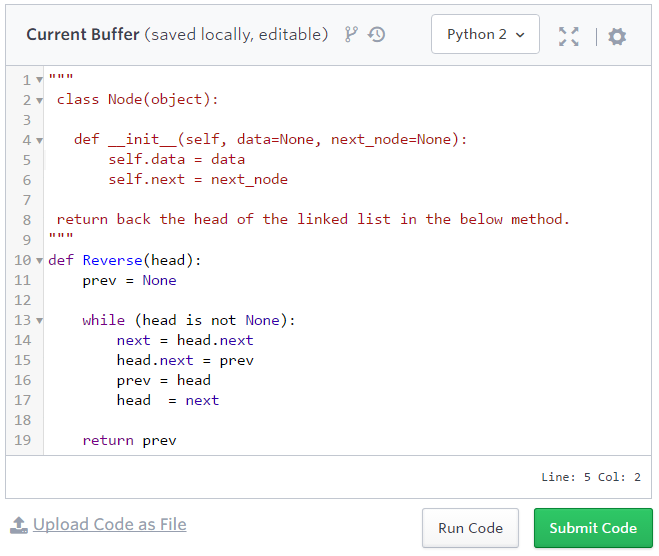
\includegraphics[width=\textwidth, trim=20 20 0 30]{img/hackerrank.png}
        \captionsetup{width=\textwidth, justification=centering}
        \captionof{figure}{Code editor from HackerRank\cite{hrlinkedlist}}\label{fig:hrlinkedlist}
      \end{minipage}%
      \quad
      \begin{minipage}{.48\textwidth}
        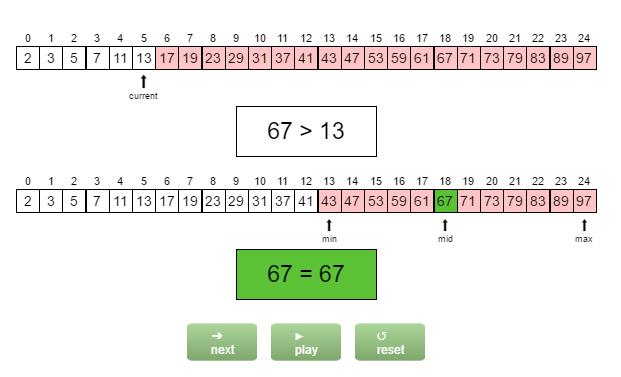
\includegraphics[width=\textwidth, trim=0 -37 0 -37]{img/khansearch.png}
        \captionsetup{width=\textwidth, justification=centering}
        \captionof{figure}{Binary search visualisation from Khan Academy\cite{khanbinsearch}}\label{fig:khanbinsearch}
      \end{minipage}
    \end{figure}

    \section{Simulators as a Teaching Aid}

    In his article {\em Evaluating A System Simulator For Computer
      Architecture Teaching And Learning Support}\cite{mustafa2010},
    Mustafa discusses the design \& implementation of a system
    which integrates the simulation of a compiler, CPU and operating
    system to aid in the teaching of undergraduate computer
    architecture and operating systems modules.

    Although brief, the article provides valuable insight into the
    design and evaluation of such teaching software. The primary
    source of feedback came from an opinion survey using a 5-point
    \gls{likertscale} for quantitative analysis and open-ended questions
    for qualitative feedback. In addition, students were administered
    a test to assess their knowledge pre- and post- use of the system.

    The evaluation results highlight an important point to consider
    when designing teaching software; over 20\% of respondents
    indicated that they spent more time learning how to use the
    software than they did completing the given exercises. An equal
    number of students reported that the simulator left them more
    confused than before. In addition, 7.1\% of respondents said that
    the simulator was too complicated to use effectively in their
    tutorials.

    However, the converse of these results gives a positive outlook
    for this project: 72.4\% of respondents disagreed with the above
    statements and 79.3\% believed that the system improved their
    understanding of the topics covered in lectures. Over 95\% of
    responents agreed that the simulator was more useful than reading
    textbooks or searching the internet in helping them understand the
    material.

    \section{Learning and Teaching Styles}

    A 1988 report by Richard M. Felder and Linda K. Silverman,
    entitled {\em Learning and Teaching Styles in Engineering
      Education}\cite{felder1988}, categorizes students' learning
    methods and describes ways in which professors may target specific
    categories in their teaching strategy.

    Felder refers to the learning modalities (or VAK) model proposed
    by Walter Burke Barbe, which defines three modalities:

    \begin{itemize}
    \item {\bf visual} -- those who learn best by viewing images and
      diagrams;
    \item {\bf auditory} -- those who learn best by listening or
      speaking aloud; and
    \item {\bf kinaesthetic} -- those who learn best by actively
      experiencing things, learning by doing.
    \end{itemize}

    The report claims that most people of college age and above, the
    intended audience of this project, identify as {\em visual}
    learners -- those who benefit from charts, diagrams and such. In
    contrast, the presentation of content in university courses is
    primarily {\em auditory} (via lectures) or a visual representation
    of auditory information (i.e. words or mathematical formulae).

    The survey results from Mustafa\cite[p. 103]{mustafa2010} support this
    observation: although only a small sample (N=54) responded, 31\%
    of respondents identified as visual learners, while a mere 6\%
    identified as auditory learners. The majority of students (52\%)
    identified as kinaesthetic learners, indicating that taking a
    hands-on approach is a valuable tool for learning.

    It should be noted that Felder discounts kinaesthetic learning
    from his report as he considers the {\em learning by doing} to be
    a separate category, perceiving the remaining attributes of
    kinaesthetic learning to have little value in engineering. A later
    observation by Felder agrees with Mustafa, stating that engineers
    are ``more likely to be active than reflective learners''
    \cite[p. 678]{felder1988}.

        \subsection{Ability to Identify Own Learning Style}

        In her PhD dissertation {\em ``Individual Differences in
          Learning: Predicting One's More Effective Learning
          Modality''} \cite{farr1970}, Beatrice J. Farr claims that
        students are able to accurately predict the learning style in
        which they perform best:

        \begin{quote}
          ``An experiment with 72 college students confirmed that
          individuals could accurately predict the modality in which
          they could demonstrate superior learning performance. The
          data also revealed that it is advantageous to learn and be
          tested in the same modality and that such an advantage is
          reduced when learning and testing are both conducted in an
          individual's preferred modality.''\cite[p. 242]{dunn1979}
        \end{quote}

        Coffield\cite[p. 120]{coffield2004} disagrees with this, based
        on an observation by Merrill\cite{merrill2000} that ``most
        students are unaware of their learning styles and so, if they
        are left to their own devices, they are most unlikely to start
        learning in new ways''. This would indicate that basing
        teaching methods on a student's preferences is damaging to
        their education. This is, however, a misinterpretation; the
        actual text of Merrill reads:

        \begin{quote}
          ``... a student must engage in those activities ... that are
          required for them to acquire a particular kind of knowledge
          or skill ... Most students are unaware of these fundamental
          instructional (learning) strategies and hence left to their
          own are unlikely to engage in learning activities most
          appropriate for acquiring a particular kind of knowledge or
          skill.''\cite[p. 4]{merrill2000}
        \end{quote}

        Merrill later argues that the optimal strategy for teaching is
        decided first and foremost by the content being taught, then
        fine-tuned to the learner's preferred style
        \cite[p. 4]{merrill2000}. By not knowing the most effective
        strategy for learning the content they are studying, a student
        limits his or her potential. However, the appropriate strategy
        {\em should} in fact be tailored to the student's preferred
        learning style to obtain the best results.

        \subsection{Criticism of Learning Modalities}\label{sec:matching}

        Some of the criticism levied at the concept of learning styles
        is that the idea of {\em matching} -- exclusively teaching a
        student based on his or her preferred learning style -- is
        harmful to a student's education. Although Coffield's
        \cite[p. 120]{coffield2004} reasoning is flawed, the
        conclusion drawn by him and Merrill \cite[p. 4]{merrill2000}
        is sound: by allowing students to exclusively use their
        preferred way of learning, students are at risk of missing out
        on more effective methods of study.

        Felder's report mentions a study carried out by the
        Socony-Vacuum Oil Company, which concludes that:

        \begin{quote}
          ``...students retain 10 percent of what they read, 26
          percent of what they hear, 30 percent of what they see, 50
          percent of what they see and hear, 70 percent of what they
          say, and 90 percent of what they say as they do
          something.''\cite[p. 677]{felder1988}
        \end{quote}

        This indicates that by relying solely upon auditory methods,
        professors can only hope to convey as little as 26\% of the
        desired material to their students. Felder advocates using a
        mixture of teaching methods in order to appeal to all
        students' preferred learning styles.

    \section{Summary}

    While there may be some disagreement over the validity of learning
    styles or modalities, even its critics seem to agree that there is
    value in varying the methods of teaching in use. At present, the
    only available resources for learning \gls{dataflowanalysis} are
    lecture slides, videos and textbooks. These are mostly auditory
    and sometimes visual methods of teaching, with little kinaesthetic
    learning involved. There is a clear need for more active study;
    although 52\% of students identified as learning best through
    kinaesthetic learning\cite[p. 103]{mustafa2010}, there is almost
    no support for this method of study.

    Given the relative success of the examples discussed in this
    chapter and the apparent lack of any such resources for
    \gls{dataflowanalysis}, there is a strong precedent for this
    project and as such a system will be developed to fulfil this
    role.

    However, it is important to note the mistakes made by the examples
    discussed here. The simulator designed by Mustafa was deemed too
    complex\cite[p. 103]{mustafa2010} and a detriment to their
    learning by over 20\% of respondents. This project will seek to
    ensure that that content is clear and concise on order to produce
    an effective learning resource.

    To evaluate the success of the system this project will build upon
    the methods presented by Mustafa, aggregating opinion using a
    \gls{likertscale} and examining this data to judge overall
    satisfaction with the software and identify specific areas for
    improvement.


\chapter{Design}
This chapter discusses the high-level design and architecture of the
system, including motivations for design choices and solutions to
conceptual problems.

    \section{Introduction}
    The original goal of this project was to produce an online
    simulation of \gls{dataflowanalysis} to show students how
    data-flow works. As discovered in the related reading, however, a
    large portion of users of a similar system found it to be too
    complex and claimed to have spent more time studying the software
    itself than the topic at hand. The literature also raised another
    key point; a wide variety of learning techniques are necessary to
    gain a true understanding of a topic.

    For these reasons the proposal has been extended to create a
    comprehensive learning platform. In addition to the simulator the
    software will provide supporting lectures to explain the basic
    concepts and gradually introduce each element of the
    simulation. These lectures will include visual and interactive
    elements to engage the user through a range of learning styles. It
    is hoped that the system will prove a valuable tool for learning
    alongside existing resources such as textbooks and lectures.

    \section{Design Constraints}
    In this section, design constraints are identified and potential
    solutions are suggested.

        \subsection{Technical Constraints}
        As the intention isto make such a system available to
        \gls{copt} students via the University, the following
        technical considerations must be made:

        \begin{itemize}
        \item The system must be distributed to all students in some format;
        \item This format must be functional on and compatible with a
          wide range of devices owned by said students;
        \item The system must be secure and require little
          maintenance; and
        \item The system must be hosted on some platform available to
          the University.
        \end{itemize}

        In order to meet these criteria the system must rely on as
        little technology as possible. The easier the platform is to
        host and distribute, the more likely it is to be made
        available to students -- a system which uses new technology
        and requires its own dedicated hosting would be more difficult
        to set up and maintain than one which can be deployed to
        existing hardware. It is necessary to ensure that the system
        is secure to avoid damaging University or student property.

        The application could be developed using purely client-side
        technologies such as JavaScript, HTML and CSS. These static
        files may be distributed over HTTP using any standard web
        server such as the one already used to host the course
        webpage. Efforts must be made to keep the performance of the
        system consistent across a range of web browsers and devices;
        although all modern web browsers are capable of interpreting
        these types of content there are subtle differences which may
        break functionality on one platform but not others.

        Use of popular libraries and frameworks such as jQuery and
        Bootstrap will be encouraged as this provides a number of
        benefits. The user will experience reduced load times since
        they have likely already downloaded the required files, and
        such libraries will provide security and robustness due to
        their wide use and active development. Likewise, the more
        popular a library is the more documentation and resources will
        be available to aid in developing the best possible system.
        
        The specific technologies used in each are detailed in
        the implementation (chapters \ref{chap:impl-simulation},
        \ref{chap:impl-visualisation} \& \ref{chap:impl-teaching}).

          
        \subsection{Content Constraints}
        To be viable as a learning platform, the system must:
        
        \begin{itemize}
        \item Appeal to a range of learning styles;
        \item Provide comprehensive coverage of the topic at hand;
        \item Ensure the content included is correct, clear and
          concise; and
        \item Maintain a shallow learning curve, gradually introducing
          students to each topic or element of the simulation.
        \end{itemize}

        Extending the proposed system into a comprehensive learning
        platform will provide a range of ways in which to study
        \gls{dataflowanalysis}. Students will have the choice to use
        the areas of the software which most appeal to them and
        content will be presented using a mixture of interactive,
        visual and textual formats.

        As the aim is to assist students of the \gls{copt} course,
        coverage of topics will be prioritised based on their
        inclusion in the course syllabus and whether they are required
        to understand the simulation:

        \begin{itemize}
        \item Basic principles of data-flow analysis;
        \item A few simple data-flows, including:
          \begin{itemize}
          \item Reaching Definitions
          \item Liveness Analysis
          \item Available Expressions
          \end{itemize}
        \item Round-robin fixed-point algorithm;
        \item Effect of orderings on analysis efficiency;
        \item Generic frameworks for data-flow analysis;
        \item Hasse diagrams and lattice representation of values; and
        \item Conditions for analysis termination.
        \end{itemize}        

        If the content delivered by the platform is incomplete,
        incorrect or too difficult to understand, the system will not
        present a viable alternative method of study. When evaluating
        the system it will be important to assess the clarity and
        presentation of the material, and the ease of use of the
        platform as a whole.


    \section{System Architecture}
    This system will be divided into three main sections:

    \begin{itemize}
    \item A \gls{dataflowanalysis} simulator, which controls the logic
      and state behind an analysis;
    \item Visual components which display the state of the
      simulation and allow users to interface with it; and
    \item Interactive components such as navigation, text pages,
      simulation controls and answerable questions.
    \end{itemize}

    The simulator forms the back-end of the system -- that is,
    elements not directly visible to the user. The front-end
    components will expose elements of the back-end, visualising the
    state of the simulation and allowing the user to interact with
    it. See fig. \ref{fig:sysarch} for a visual representation.
    
    Object-oriented design will be paramount, allowing functionality
    to be extended and shared between similar elements. In addition to
    speeding up development of the system by reducing the need to
    duplicate code, this is generally good design practice. Components
    will be written as re-usable modules which can be combined in
    different ways, for example to present the user with a series of
    lectures or an interactive simulation. See
    \S\ref{sec:design-interface} for more details on the user
    interface.
   
    \begin{figure}[!ht]
      \centering
      \scalebox{0.8}{
        \begin{tikzpicture}[x=1mm, y=-1mm,
          person/.pic={%
            \node (-head) [circle, minimum size=4*\pgfkeysvalueof{/cfr/soul base dimension}] {};
            \node (-torso) [below=0pt of -head, rectangle, rounded corners=.4*\pgfkeysvalueof{/cfr/soul base dimension}, minimum width=3.5*\pgfkeysvalueof{/cfr/soul base dimension}, minimum height=6*\pgfkeysvalueof{/cfr/soul base dimension}] {};
            \node (-right arm) [right=0pt of -torso.north east, yshift=-3.1*\pgfkeysvalueof{/cfr/soul base dimension}, rectangle, minimum width=\pgfkeysvalueof{/cfr/soul base dimension}, minimum height=6*\pgfkeysvalueof{/cfr/soul base dimension}, rounded corners=.4*\pgfkeysvalueof{/cfr/soul base dimension}] {};
            \node (-left arm) [left=0pt of -torso.north west, yshift=-3.1*\pgfkeysvalueof{/cfr/soul base dimension}, rectangle, minimum width=\pgfkeysvalueof{/cfr/soul base dimension}, minimum height=6*\pgfkeysvalueof{/cfr/soul base dimension}, rounded corners=.4*\pgfkeysvalueof{/cfr/soul base dimension}] {};
            \node (-left leg) [below=0pt of -torso.south, rectangle, minimum width=1.5*\pgfkeysvalueof{/cfr/soul base dimension}, minimum height=6*\pgfkeysvalueof{/cfr/soul base dimension}, rounded corners=.2*\pgfkeysvalueof{/cfr/soul base dimension}, anchor=north east] {};
            \node (-right leg) [below=0pt of -torso.south, rectangle, minimum width=1.5*\pgfkeysvalueof{/cfr/soul base dimension}, minimum height=6*\pgfkeysvalueof{/cfr/soul base dimension}, rounded corners=.2*\pgfkeysvalueof{/cfr/soul base dimension}, anchor=north west] {};
            \draw [rounded corners=.2*\pgfkeysvalueof{/cfr/soul base dimension}] (-right leg.south) -- (-right leg.south west) -- (-left leg.south east) -- (-left leg.south west)  -- (-torso.south west) [rounded corners=.4*\pgfkeysvalueof{/cfr/soul base dimension}] -- (-left arm.south east) -- (-left arm.south west) -- (-left arm.north west) -- (-torso.north west) -- ($(-head.south) - (.5*\pgfkeysvalueof{/cfr/soul base dimension},0)$) arc [start angle=255.5, end angle=-74.5, radius=2*\pgfkeysvalueof{/cfr/soul base dimension}] -- (-torso.north east) -- (-right arm.north east) -- (-right arm.south east)  -- (-right arm.south west) [rounded corners=.2*\pgfkeysvalueof{/cfr/soul base dimension}] -- (-torso.south east)  -- (-right leg.south east) -- (-right leg.south west);
          }
          ]
          % vertices
          \tikzstyle{group} = [rectangle, draw, text centered, rounded corners, densely dotted, below right]
          \tikzstyle{cluster} = [rectangle, draw, text width=60mm, text centered, rounded corners, dashed, below right]
          \tikzstyle{clusterlabel} = [text width=60mm, minimum height=10mm, text centered, below]
          \tikzstyle{component} = [rectangle, draw, text width=50mm, text centered, rounded corners, minimum height=7mm, below right]

          \node[group, text width=135mm, minimum height=56mm] (backend) at (0,0) {};
          \node[clusterlabel, text width=100mm] at (backend.north) {Back-end Components};

          \node[cluster, minimum height=42mm, below = 10mm of backend.north] (simulator) {};
          \node[clusterlabel] at (simulator.north) {Simulator};
          \node[component, below=10mm of simulator.north] (sfwk)  {Data-Flow Framework};
          \node[component, below=20mm of simulator.north] (scfg)  {Program CFG};
          \node[component, below=30mm of simulator.north] (salgo) {Analysis Algorithm};

          \node[group, text width=135mm, minimum height=76mm, below=5mm of backend.south] (frontend) {};
          \node[clusterlabel, text width=100mm] at (frontend.north) {Front-end Components};

          \node[cluster, minimum height=62mm, below left=10mm and 2mm of frontend.north] (visual) {};
          \node[clusterlabel] at (visual.north) {Visual Components};
          \node[component, below=10mm of visual.north] (vcfg)   {Visual CFG};
          \node[component, below=20mm of visual.north] (vhasse) {Hasse Diagram};
          \node[component, below=30mm of visual.north] (vres)   {Table of Results};
          \node[component, below=40mm of visual.north] (vlst)   {Code Listing};
          \node[component, below=50mm of visual.north] (vfwk)   {Framework Properties};

          \node[cluster, minimum height=52mm, below right=10mm and 2mm of frontend.north] (interface) {};
          \node[clusterlabel] at (interface.north) {Interactive Components};
          \node[component, below=10mm of interface.north] (imenu) {Navigation};
          \node[component, below=20mm of interface.north] (itext) {Text Pages};
          \node[component, below=30mm of interface.north] (iques) {Questions};
          \node[component, below=40mm of interface.north] (icont) {Simulation Controls};
          
          \pgfkeyssetvalue{/cfr/soul base dimension}{5pt}
          \pic (user) [below=5mm of frontend.south] {person};

          % \draw[edge] (simulator) .. controls ([xshift=-4cm] simulator) and ([xshift=4cm] visual) .. (visual);

          \draw[-{>[scale=2.5]}] ($ (interface.north) + (8, 0) $) |- (simulator.east) node [near start, right, text width=30mm, text centered] {\footnotesize User actions update simulation};
          \draw[-{>[scale=2.5]}] (simulator.west) -| ($ (visual.north) +  (-8, 0) $) node [near end, left, text width=25mm, text centered] {\footnotesize Updates propagated to visual components};
          \draw[-{>[scale=2.5]}] ($ (user-right arm.east) + (2, 0)$) -| ($ (interface.south) + (8,0) $) node [midway, above right, text width=28mm, text centered] {\footnotesize User interacts with front-end};
          \draw[-{>[scale=2.5]}] ($ (visual.south) + (-8, 0) $) |- ($ (user-left arm.west) + (-2, 0)$) node [midway, above left, text width=28mm, text centered] {\footnotesize User receives visual feedback};
        \end{tikzpicture}
      }
      \captionsetup{justification=centering}
      \caption{An overview of the planned system architecture.}\label{fig:sysarch}
    \end{figure}


    \section{User Interface Design}\label{sec:design-interface}

    

    \section{Data Collection}

    To evaluate the system anonymous usage data will be collected. A
    variety of web platforms exist for this purpose including Google
    Analytics and Piwik. However, these platforms are intended for
    large-scale data collection and as such are not suited for the
    fine-grained analysis necessary in the evaluation of this
    project. As an example, it is not possible to link tracked events
    to specific users or view a complete list of triggered events
    using Google Analytics. Furthermore, extended use of these
    platforms often comes at significant financial cost. It is also
    important to consider the ethical issues that may arise from
    sharing usage data with companies like Google; using such a
    platform would require a much deeper discussion around user
    privacy and use of the data for financial gain.

    Developing a custom event-tracking \gls{api} would allow full
    control of the data collected both in terms of accessing the raw
    data and maintaining user privacy.

    The data model must be able to store the following on a per-user
    basis:

    \begin{itemize}
    \item Page views;
    \item Button clicks and interactions with components;
    \item Page load times; and
    \item Question attempts and overall scores.
    \end{itemize}

    All of these can be modeled using an API with a single
    endpoint\footnote{An endpoint is a URL at which a particular API
      service may be accessed, e.g. \url{api.com/users/} may provide
      access to user data} based on the Google Analytics event
    model. Each {\tt event} record has the following fields:

    \begin{itemize}
    \item A {\tt tracking token} used to group events by user;
    \item A {\tt type} such as page view or button click;
    \item The {\tt datetime} at which the event occurred; and
    \item Four levels of categorization: {\tt category}, {\tt action},
      {\tt label}, and {\tt value}. Each field can be used to group
      similar events and store values such as question scores or which
      element was clicked. The actual content of these fields does not
      matter as long as the grouping is consistent.
    \end{itemize}

    The tracking token will be generated when the user first visits
    the page and persist across visits to the site. Storing this token
    will enable analysis of how a user's actions affect their
    achievement of learning outcomes, such as whether completing a
    given tutorial or using a simulator component increases question
    scores in the related topic. It will be possible to determine
    which elements of the software users find difficult to understand
    based on their interactions with each component.
    

%%%%%%%%%%%%%%%%%%%%%%%%%%%%%%%%%%%%%%%
\chapter{Data-Flow Analysis Simulation}\label{chap:impl-simulation}
This chapter discusses the implementation of the
\gls{dataflowanalysis} simulation -- the back-end elements which
control the logic and state of the analysis, which is then interpreted
by the visual elements described in chapter
\ref{chap:impl-visualisation}.

    \section{Overview}
    The implementation of the simulator is based upon the concept of a
    general framework as described in
    \S\ref{sec:background-frameworks} of this report and \S10.11 of
    the {\em Dragon Book}\cite{dragonbook}. The simulator takes as
    input a program written in the ILOC language, a \gls{dataflow}
    framework and an order in which to evaluate nodes. It parses the
    program into an \gls{ast} and uses this to build a \gls{cfg}, then
    performs an analysis on said graph using the round-robin
    \gls{fixedpoint} algorithm for general frameworks (algorithm
    \ref{algo:general}).

    Playback of the simulation can be controlled through the
    simulator's \gls{api}. Function calls which update the state of
    the simulation trigger an event handling system to update the
    visual components. However, the simulation is entirely independent
    of the rest of the system; re-using it in another project is as
    simple as copying the directory containing the simulator code and
    including the required libraries.

    The simulator is implemented entirely in JavaScript and makes use
    of some jQuery features and a set of helper functions gathered
    from sources such as StackOverflow. Snippets of code taken from
    external sources are explicitly commented as such in the source
    code and will be mentioned here.

    \section{Value Sets}

    JavaScript includes a native {\tt Set} data structure for
    representing collections of unique objects. Unfortunately, two
    objects are only seen as equal if they refer to the exact same
    instance. For the purposes of this simulation it would be useful
    to compare objects which share some attributes but refer to
    different instances; for example, when operating on sets of
    operands it would be useful to consider two operands of different
    instructions as the same if they refer to the same variable.

    For this reason the simulator uses a new {\tt ValueSet} data
    structure, backed by a native JavaScript {\tt Map}. The {\tt
      ValueSet} stores objects which inherit from a {\tt
      ValueMixin}\footnote{A mixin class contains methods which may be
      inherited by another class, but is not necessarily the parent of
      that class.}, which defines a {\tt key} function to obtain a
    unique identifier for a given object. Objects are checked for
    equality using this identifier, so that two objects may be
    considered equal based on selected attributes.

    The {\tt ValueSet} supports the following operations, with
    estimated time complexities based on the description of {\tt Map}s
    in the \gls{es6} specification\cite{es6-maps}:

    \begin{figure}[!ht]
      \centering
      \begin{tabular}{|c|c|c|c|c|c|}
        \hline
        size   & add    & delete & has    & union  & intersect \\ \hline
        $O(1)$ & $O(1)$ & $O(1)$ & $O(1)$ & $O(n)$ & $O(n)$    \\ \hline
      \end{tabular}
    \end{figure}

    

    \section{Data-Flow Framework}
    
    Each data-flow framework defines the elements outlined in
    \S\ref{sec:background-frameworks}, namely:

    \begin{itemize}
    \item The {\em \gls{domain}} of values on which to operate;
    \item The {\em \gls{direction}} in which data flows;
    \item A set of {\em \gls{dataflowequations}} including the {\em
        \gls{meetoperator}} $\land$ and the set of {\em
        \gls{transfer} functions} $F$.
    \item The {\em \gls{boundary}} value specifying the initial value
      at the entry or exit to the \gls{cfg}; and
    \item The {\em initial value}, $\top$, at each point in the graph.
    \end{itemize}

    The meet and transfer functions operate on {\tt
      ValueSets}. Frameworks must also specify the following additional
    information:

    \begin{itemize}
      \item
    \end{itemize}

    \section{Algorithms for Analysis}
    Blah Blah
    
        \subsection{Iterative Algorithm}
        Blah Blah
    
    \section{Intermediate Language for Optimising Compilers}
    Blah Blah
    
        \subsection{Parsing Expression Grammar}
        Blah Blah
    
        \subsection{Control-Flow Graphs}
        Blah Blah


%%%%%%%%%%%%%%%%%%%%%%%%%%%%%%%%%%%%%%%
\chapter{Data-Flow Analysis Visualisation}\label{chap:impl-visualisation}
Blah Blah

    \section{Data-Flow Framework}
    Blah Blah
    
    \section{Simulator}
    Blah Blah
    
    \section{Control-Flow Graph}
    Blah Blah
    
    \section{Lattice}
    Blah Blah
    

%%%%%%%%%%%%%%%%%%%%%%%%%%%%%%%%%%%%%%%
\chapter{Interactive Learning}\label{chap:impl-teaching}

    \section{User-defined Programs}
    Blah Blah
    
    \section{Interactive Tutorials}
    Blah Blah
    
    \section{Experimental Sandbox}
    Blah Blah
    

%%%%%%%%%%%%%%%%%%%%%%%%%%%%%%%%%%%%%%%
\chapter{Evaluation}
Blah Blah

% use the following and \cite{} as above if you use BibTeX
% otherwise generate bibtem entries
\bibliographystyle{unsrtnat}
\bibliography{mybibfile}

\begin{appendices}

\chapter{Terminology}\label{appx:glossary}

\printglossaries

\chapter{Types of Data-Flow Analysis}\label{appx:analysistypes}

\bgroup
  \vspace{-5mm}
  \begin{tabular}{|l|p{5cm}|p{5cm}|}
    \hline
    {\bf Data-Flow}                         & {\bf Purpose}                                                                                              & {\bf Applications}                                                                              \\ \hline
    Dominators                              & Computes the set of nodes which \gls{dominate} the current node.                                           & Computing SSA form.                                                                             \\ \hline
    \Gls{reachingdefinition}s               & Computes the set of variable definitions which are available at points in the CFG.                         & Generating def-use chains for other analyses.                                                   \\ \hline
    \Gls{livenessanalysis}                  & Computes the set of variables whose current value will be used at a later point in the control flow graph. & Register allocation. Identifying useless store operations. Identifying uninitialised variables. \\ \hline
    \Gls{availableexpression}s              & Identifies expressions which been computed at a previous point in the CFG.                                 & Code motion.                                                                                    \\ \hline
    Anticipable Expressions                 & Computes expressions which will be computed along all paths leading from the current point.                & Code motion.                                                                                    \\ \hline
    Constant Propagation                    & Computes the set of variables which have a constant value based on previous assignments.                   & Constant propagation. Dead code elimination.                                                    \\ \hline
    Copy Propagation                        & Computes the set of variables whose values have been copied from another variable.                         & Dead code elimination. Code motion.                                                             \\ \hline
    Tainted Flow Analysis\cite{TaintedFlow} & Identifies unsafe operations which have been passed unsanitized {\em (tainted)} input as a parameter.      & Preventing security vulnerabilities such as SQL injection and XSS attacks.                      \\ \hline
  \end{tabular}
  \captionof{table}{Types of data-flow analysis.}
\egroup


\end{appendices}

\end{document}
